\documentclass[12pt]{article}
\usepackage[utf8]{inputenc}

% No indent
\setlength\parindent{0pt}
% Paragraph spacing
\setlength{\parskip}{0.4cm}

\usepackage[table,xcdraw]{xcolor}
\usepackage{changepage}
\usepackage{booktabs,amssymb,makecell,rotating}
\usepackage{caption}
% Page Layout
\usepackage{fancyhdr}
\pagestyle{fancy}
\fancyhf{}
\fancyhead[RE,LO]{\leftmark}
\fancyfoot[LE,RO]{\thepage}
% Packages to manage images
\usepackage{graphicx}
\usepackage[section]{placeins}
\usepackage[skip=15pt]{caption}
\usepackage{subcaption}
% Packages to manage tables
\usepackage{tabu}

% Package for hyperlinks
\usepackage{hyperref}
\hypersetup{colorlinks,urlcolor=blue}
% Path to the images
\graphicspath{{images/}}


% Title
\title{TrackMe Software Design Document}
% Authors
\author{Andrea Biscontini, Marco Gelli, Alvise de' Faveri Tron}
% Date
\date{Dec 2018}

\makeatletter
\let\thetitle\@title
\let\theauthor\@author
\let\thedate\@date
\makeatother

\begin{document}

\begin{titlepage}
	\centering
	\vspace*{0.5 cm}
	
\includegraphics[scale = 0.75]{logopoli}\\[1.0 cm]	% University Logo
	\textsc{\LARGE MSc in Computer Science and Engineering}\\[2.0 cm]	% University Name
	\textsc{\Large Software Engineering 2 Project}\\[0.5 cm]				% Course Code
	\rule{\linewidth}{0.2 mm} \\[0.4 cm]
	{ \huge \bfseries \thetitle}\\
	\rule{\linewidth}{0.2 mm} \\[1.5 cm]
	
	\begin{minipage}{0.4\textwidth}
		\begin{flushleft} \large
			\emph{Professor:}\\
			Elisabetta di Nitto\\
		\end{flushleft}
	\end{minipage}~
	\begin{minipage}{0.6\textwidth}
		
		\begin{flushright} \large
			\emph{Authors :} \\
			Andrea Biscontini - 901310\\
			Marco Gelli - 901470\\
			Alvise de'Faveri Tron - 920882\\
		\end{flushright}
		
	\end{minipage}
		
\end{titlepage}

\newpage

\tableofcontents

\section{Introduction}
prima dei sottocapitoli
\subsection{Purpose}
This document represent the Requirement Analysis and Specification Document of the Data4Help system. Here it's described the general purpose of the system, the functional and non-functional requirements that it must respect and the assumption through which we achieve all it's goal. This document is addressed to all the stakeholder of this system, which means final clients but also management, developer, testers and more.\\
The Data4Help system is composed by an user side smartphone Application and a web based query service for the third parties. The user-side App has the task to collect data from all the devices connected to the user's smartphone and send them to the TrackMe database. The web service is instead used by third parties to submit data request to TrackMe and, if they are successful, receive the most recent data collected on the proprietary databases.
AutomatedSOS is instead an user-side integration for the Data4Help service. Registered users' real time data are here monitored and, if there is any signal of possible health problems, local emergency numbers are called and an ambulance is called to intervene at the customer location.
Track4Run isanother ananotheranotheranotheranotherother system built upon Data4Help. Here users can become run organizers, enroll in scheduled runs and spectate live runs through a map with live GPS ranotheranotheranotherunners position.
\subsection{Scope}
\subsubsection{Description of the given problem}
As stated in the above section, Data4Help main goal is to collect user's data and made them available to third parties, all while guaranteeing the user privacy and consensus in personal data processing. To collect these data, the system needs to connect to users' smartwearables and download all the relevant produced data to TrackMe proprietary servers. Then this data are processed by TrackMe and whenever a request for data arrives from the third parties, if the request is successful, they're made available to them. Third parties could also desire to look for future changes in the data they requested, so an auxiliary subscription to new data is also made available at request time. Other than that, to simplify the data request procedure, this has been divided in two types of request: single user data request, that is forwarded directly to the individual that can accept or refuse it, and request for anonymized data of groups of individual, that is handled by TrackMe and it's always successful if there is the possibility to render the data anonym.
On top of the Data4Help system, that is used mainly by third party as a data retrieving service, there are AutomatedSOS and Track4Run. These service are instead to be used by an user of Data4Help. AutomatedSOS means is to help elderly or non-healty people to monitor their health status and intervene in the case of an emergency. In fact the goal of AutomatedSOS is to be very reactive (maximum 5 seconds) whenever a possible health problem is signaled and to immediately call emergency number and an ambulance for the location of the client.
Track4Run is instead a system designed for athletes and runners in which it's possible to organize, partecipate and spectate organized running competitions. Here any user can become the organizer of a run by creating one. The run creation procedure here is made really simple for the organizer, who needs only to insert the needed infos and select a route for the run on the map. When a run is created, every other user can enroll to it. To give an even better service, there is also the possibility to spectate a run on the App, which means follow every runner's position on a live GPS map.

The whole system ....
\subsubsection{Current System}
\subsubsection{Goals}
\begin{itemize}
\item \textbf{G1} Data4Help must be able to keep track of real time health status and position from registered users
\item \textbf{G2} Data4Help should allow third parties to gather information from a single user or from an anonymous group of users
\item \textbf{G3} Data4Help should allow third parties to subscribe to new data and receive them as soon as they're produced
\item \textbf{G4} AutomatedSOS should be able to identify an health emergency when the user data are below/exceeding a certain thresholds
\item \textbf{G5} AutomatedSOS must call an ambulance when it detects a health emergency
\item \textbf{G7} Track4Run allows a user to become an organizer of a run, so that he/she can create and manage a run
\item \textbf{G8} Track4Run allows a user to partecipate to an organized run
\item \textbf{G9} Track4Run allows a spectator to track the position of the partecipants of a run 
\end{itemize}
\subsection{Definitions, Acronyms, Abbreviations}
\subsubsection{Definitions}
third party, data source, synchronization, parameter, threshold,

\subsubsection{Acronyms}
\begin{itemize}
\item \textbf{RASD}: Requirement Analysis and Specification Document
\item \textbf{API}: Application Programming Interface
\item \textbf{GPS}: Global Positioning System
\item \textbf{GDPR}: General Data Protection Regulation
\end{itemize}

\subsubsection{Abbreviations}
\begin{itemize}
\item \textbf{D4H}: Data4Help
\item \textbf{ASOS}: AutomatedSOS
\item \textbf{T4R}: Track4Run
\item \textbf{Gn}: n-th goal
\item \textbf{Dn}: n-th domain assumption
\item \textbf{Rn}: n-th functional requirement
\end{itemize}
\subsection{Revision history}
quattro
\subsection{Reference Documents}
cinque
\subsection{Document Structure}
sei
%what you write here is a comment that is not shown in the final text

\newpage

\section{Architectural Design}
\subsection{Overview}
As stated above, each subsystem has to accomplish its own goal. In particular, we can see AutomatedSOS and Track4Run as simple, three-tier applications, while Data4Help should display a more complex, scalability-oriented architecture.

The figure below gives a general overview of a possible implementation of the system.

\FloatBarrier

\begin{figure}[!h]
	\centering
	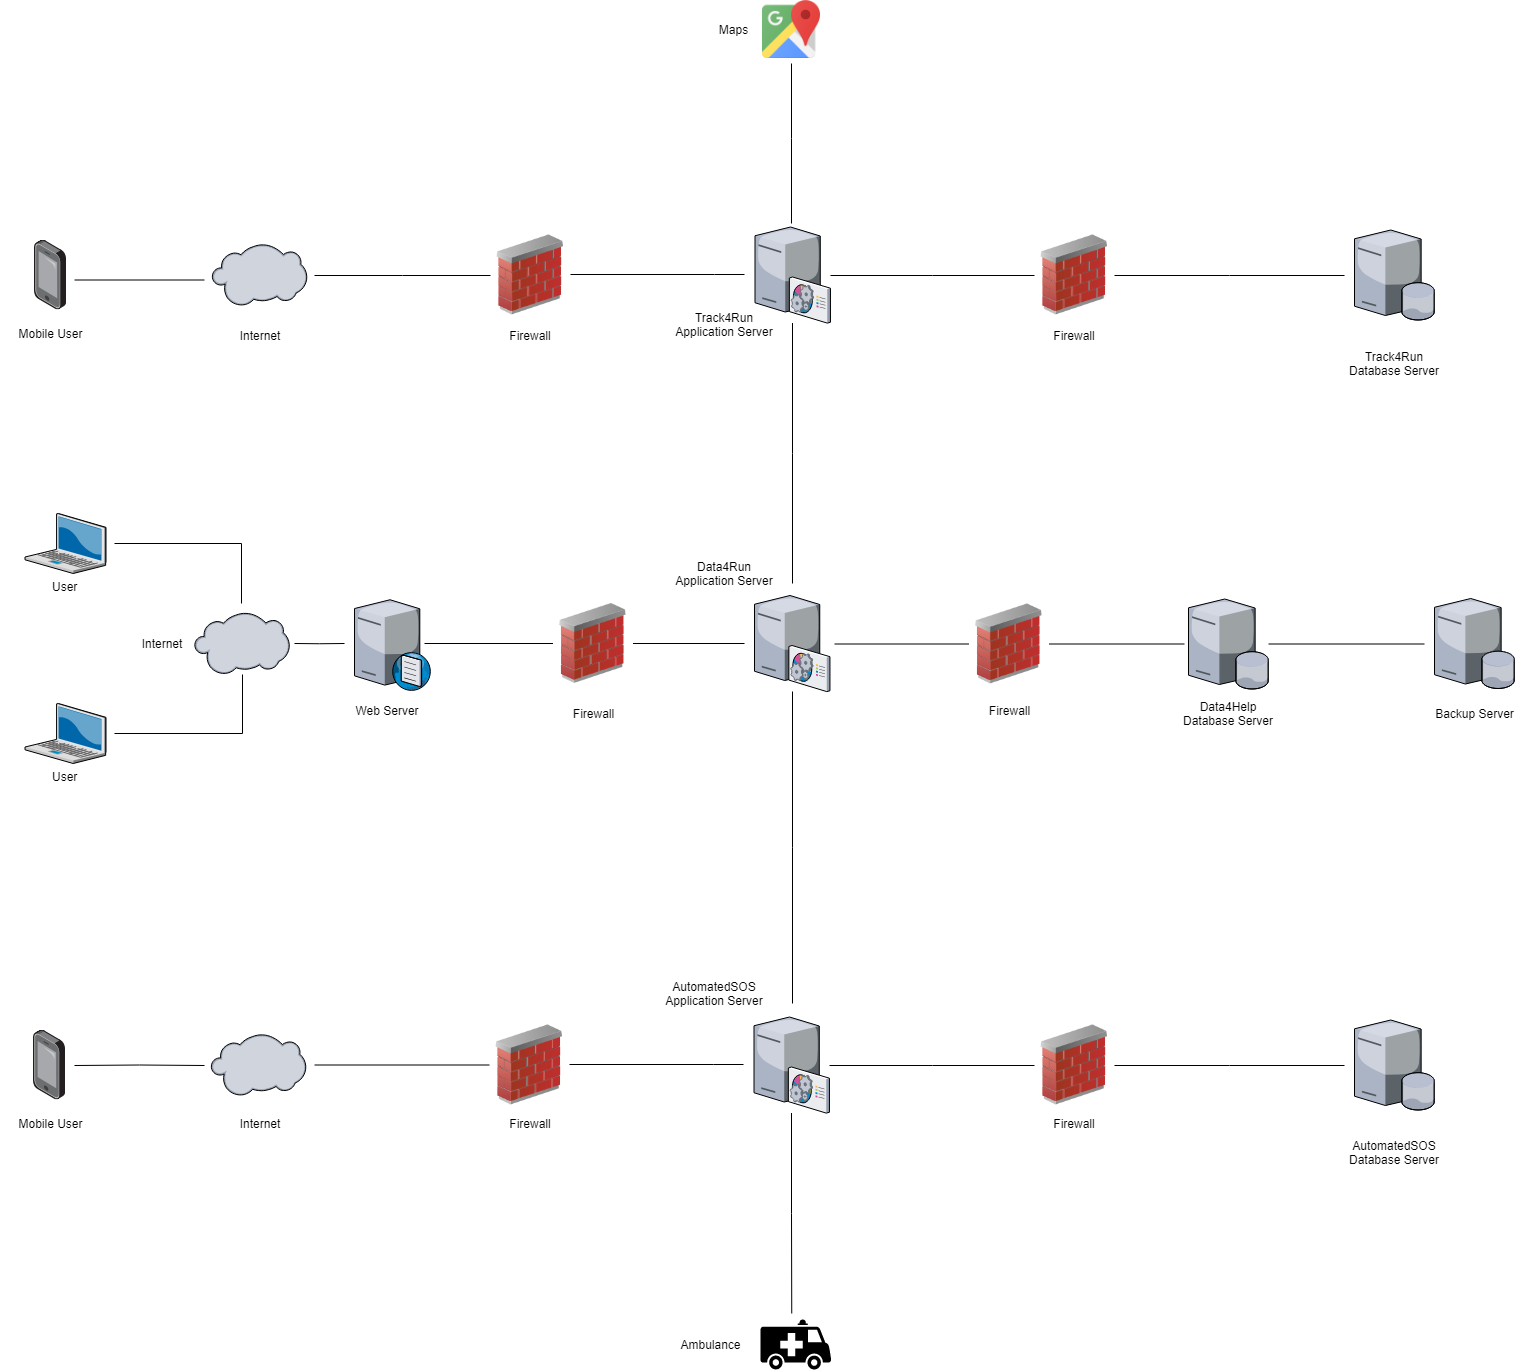
\includegraphics[width=\columnwidth]{physicalArchitectureDiagram.png}
	\caption{General Architecture}
\end{figure}


\FloatBarrier

As displayed in this figure, Data4Help subsystem's services can be accessed by many channels, including a web interface for users and APIs for data-sources and third-parties.
Since the data-sources provide real-time data from the user's devices, it is predictable that this flow of information will soon grow into a huge number of requests, so this subsystem has to be designed to quickly accomplish horizontal scaling and maintain high availability even in extreme conditions.
For this reason, a Microservice based architecture enforced with Message Queues and scalable databases should be adopted, as will be described in the following sections. Also an API Gateway is used to access all Data4Help interfaces, so to easily manage authentication and load balancing from the very first moment of any request.

AutomatedSOS and Track4Run instead are designed as applications with a thick client (i.e. smart-phone and smart-watch apps), a lightweight back-end server and a storage module. This design has been chosen because it is completely modular on one hand, since the two application's business logic is separated from Data4Help's one, but guarantees on the other hand a fast and reliable service provided by the servers, leaving the full responsibility of the presentation part to the mobile application. The separation of presentation and business logic also guarantees the maintainability of the system and good performances on mobile devices, where power consumption and CPU usage can be an issue.

\subsection{High Level Architecture}

From the component point of view, each subsystem can be divided into \textit{back-end} components, which are responsible of carrying out the business logic of the subsystem, and \textit{front-end} components, which provide a presentation layer to end users and SDKs to external developers who want to access the system's services.
Also, some external components are used to provide some of the services offered by the system.
In the following diagram, the main components and interfaces are highlighted, to give a general idea of the design of the system.
It must be noted that in this diagram components and \textit{modules} represent a set of services grouped together, and that internal interaction between modules is not shown for sake of simplicity: the complete description of all the modules and internal interfaces can be found in the following sections.

\FloatBarrier
\begin{figure}[!h]
	\centering
	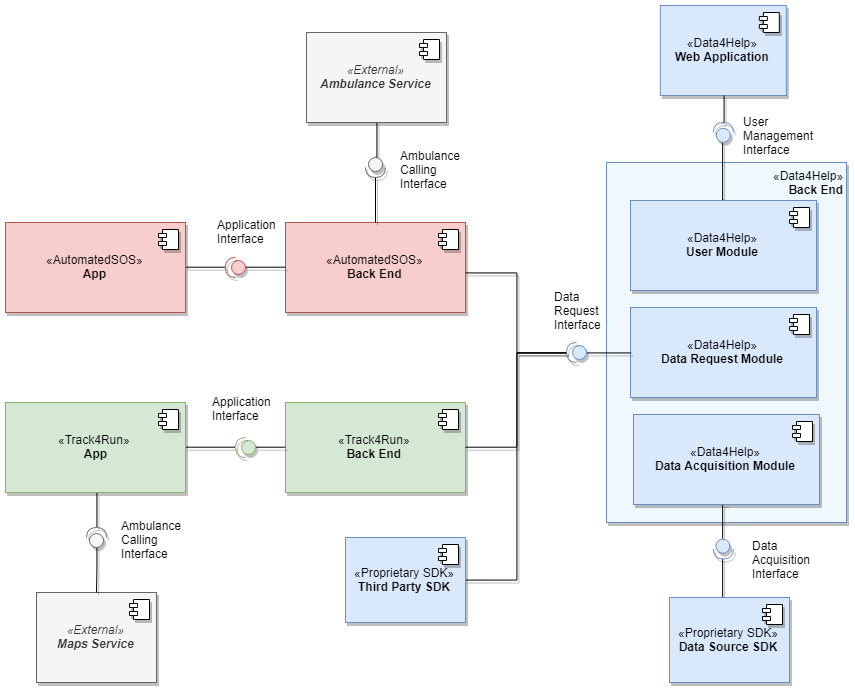
\includegraphics[width=\columnwidth]{ComponentDiagrams-Total.png}
	\caption{High Level Components}
\end{figure}
\FloatBarrier

As can be seen, the Data4Help back-end offers three main functionalities:

\begin{itemize}
	\item \textit{User Management}: provides an interface for managing the user account and configure his data-sources. This interface is exploited by a \textit{Web Application} that can be accessed via web browser.
	\item \textit{Data Acquisition}: provides the interface for collecting data from data-sources. A proprietary \textit{Data Source SDK} can be offered to external developers to integrate the use of this interface into their software and send data from external devices to Data4Help.
	\item \textit{User Management}: enables third parties to make requests on the data received by the subsystem. This interface is used by \textit{Track4Run} and \textit{AutomatedSOS} back-ends, but it can also be accessed by any other third party via the dedicated \textit{Third Party SDK}.
\end{itemize}

The other two back-ends are mainly responsible of exploiting Data4Help's serviced to offer an interface to the user's Application. 
For AutomatedSOS, an external ambulance calling interface is also needed by the back-end to fulfill its goal, while in Track4Run a Maps Service such as \textit{Google Maps} should be accessed directly from the Application to minimize latency and bandwidth occupation in the communication between the client and the server.

Another definition of the services offered by the system can be found in the figure below, which highlights the dependencies between the Data4Help system and its actors and provides a list of the services consumed internally and externally by the system.

\FloatBarrier
\begin{figure}[!h]
	\centering
	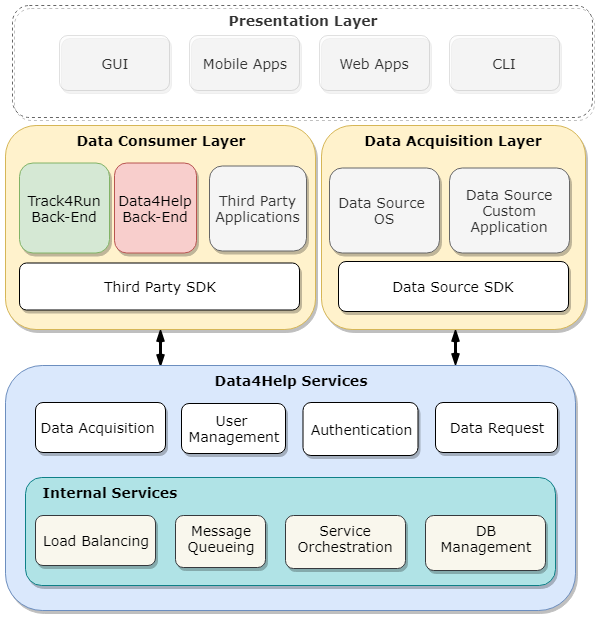
\includegraphics[width=0.8\columnwidth]{ComponentDiagrams-Layers.png}
	\caption{High Level Components}
\end{figure}
\FloatBarrier

\newpage
\subsection{Component View}


\subsubsection{Data4Help}

When considering the architecture for Data4Help, the first thing to take in account is scaling and availability. Data-sources can produce a lot of traffic, and vital services built on top of this subsystem, such as AutomatedSOS, bring the need for the system to handle all the data without losses, latency or service unavailability.
Bearing this in mind, the general idea of this subsystem's design is to exploit the new patterns of microservices and messages queues. 

The main focus of this design is that every service should be replicable in any desired number of instances (\textit{horizontal scaling}) without the need of changing other parts of the system. For this to be possible, the system must be provided with the following capabilities:

\begin{itemize}
	\item \textit{Container Environment}
	\item \textit{Container Orchestration}
	\item \textit{Load Balancing}
\end{itemize}

Future developments of the system can also add performance monitoring services, to test in real-time the stress level of the system and eventually deploy new instances of some services where needed.

This said, here is a detailed view of the components of this subsystem: each service is to be considered as independently deployed in a container, which is managed by the \textit{orchestrator}. For the sake of simplicity, only the interaction between developed components is highlighted, while the components dedicated to load balancing, orchestration and services deployment are considered to be already present as part of the \textit{API Gateway}.


\FloatBarrier
\begin{figure}[!h]
	\centering
	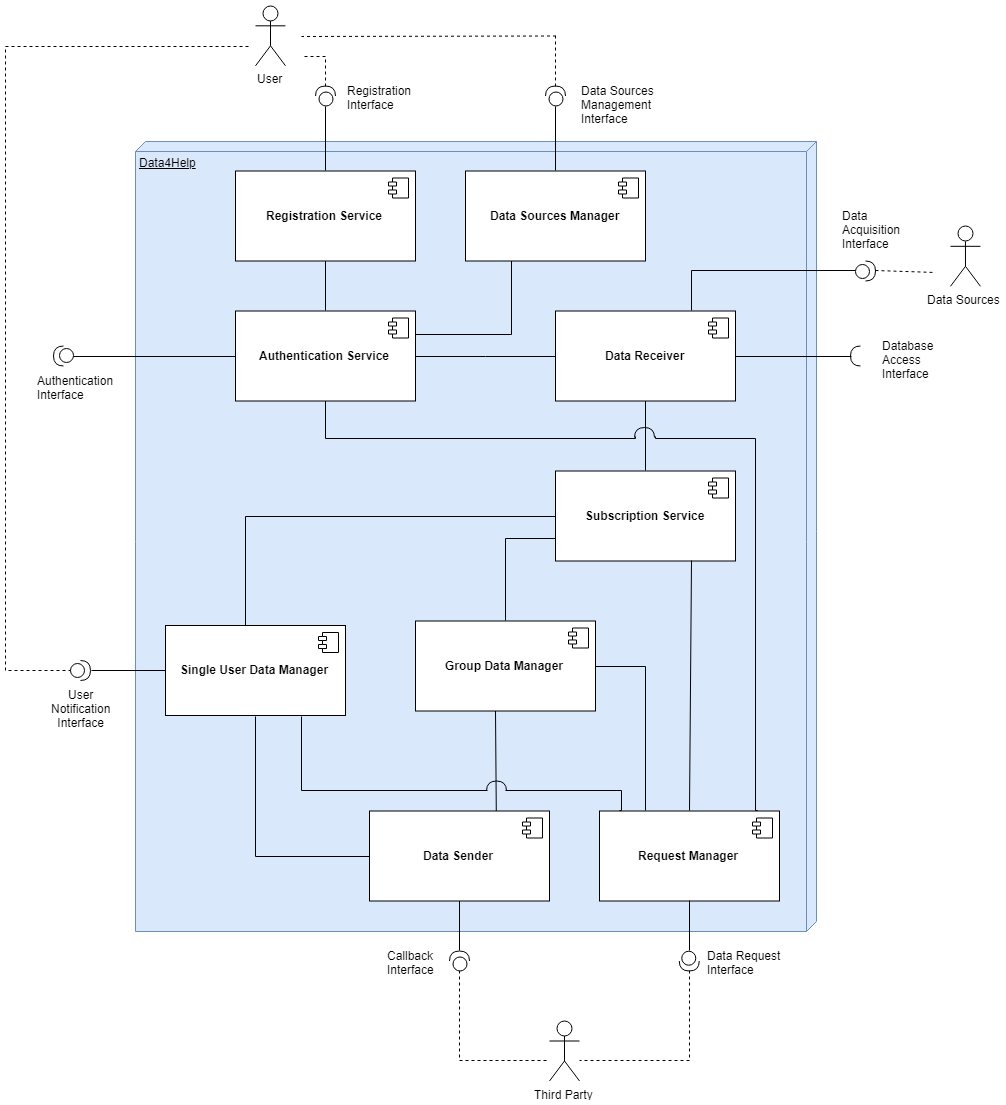
\includegraphics[width=\columnwidth]{ComponentDiagrams-Data4Help.png}
	\caption{Data4Help Components}
\end{figure}

\FloatBarrier

The internal microservices that have been identified are:
\begin{itemize}
	\item \textbf{Authentication Service}
	\item \textbf{User Service}
	\item \textbf{Receiver}
	\item \textbf{Request Manager}
	\item \textbf{Sender}
	\item \textbf{Subscription Service}
	\item \textbf{Anonymization Service}
\end{itemize}

This subsystem shall also use messaging between microservices where asyncronous communication is possible, in particular:

\begin{itemize}
	\item \textbf{New Data Queue}
	\item \textbf{New Request Queue}
	\item \textbf{Notification Queue}
	\item \textbf{Sending Queue}
\end{itemize}

All other components shall use synchronous protocols, such as RESTful APIs.

\subsubsection{AutomatedSOS}

\begin{figure}[!h]
	\centering
	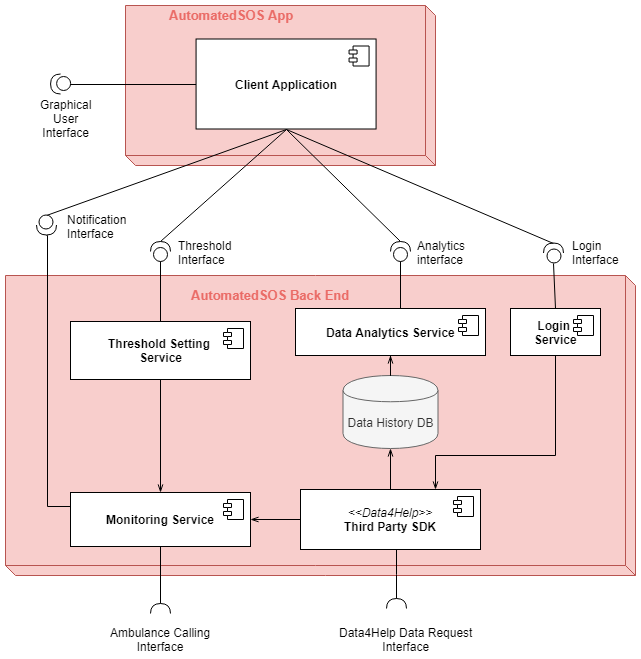
\includegraphics[width=\columnwidth]{ComponentDiagrams-AutoSOS.png}
	\caption{AutomatedSOS Components}
\end{figure}

\FloatBarrier


\subsubsection{Track4Run}

\FloatBarrier
\begin{figure}[!h]
	\centering
	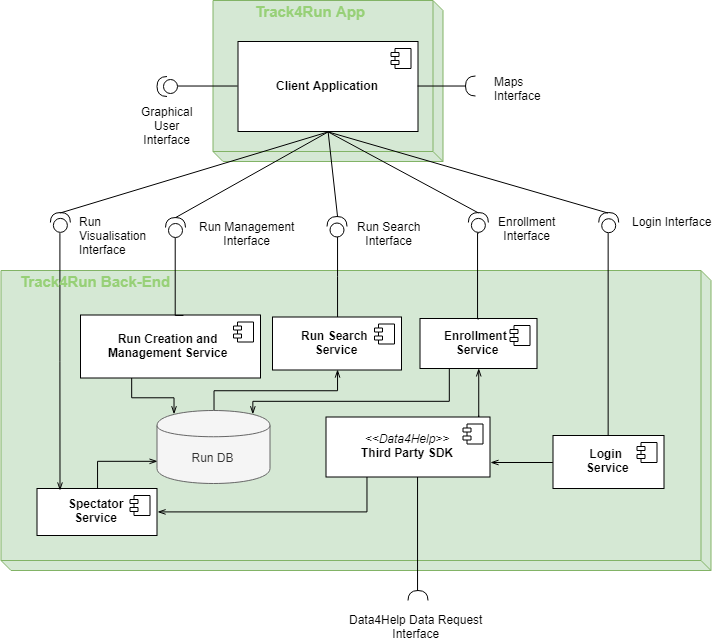
\includegraphics[width=\columnwidth]{ComponentDiagrams-Track4Run.png}
	\caption{Track4Run Components}
\end{figure}
\FloatBarrier



\subsection{Deployment View}

\FloatBarrier
\begin{figure}[!h]
	\centering
	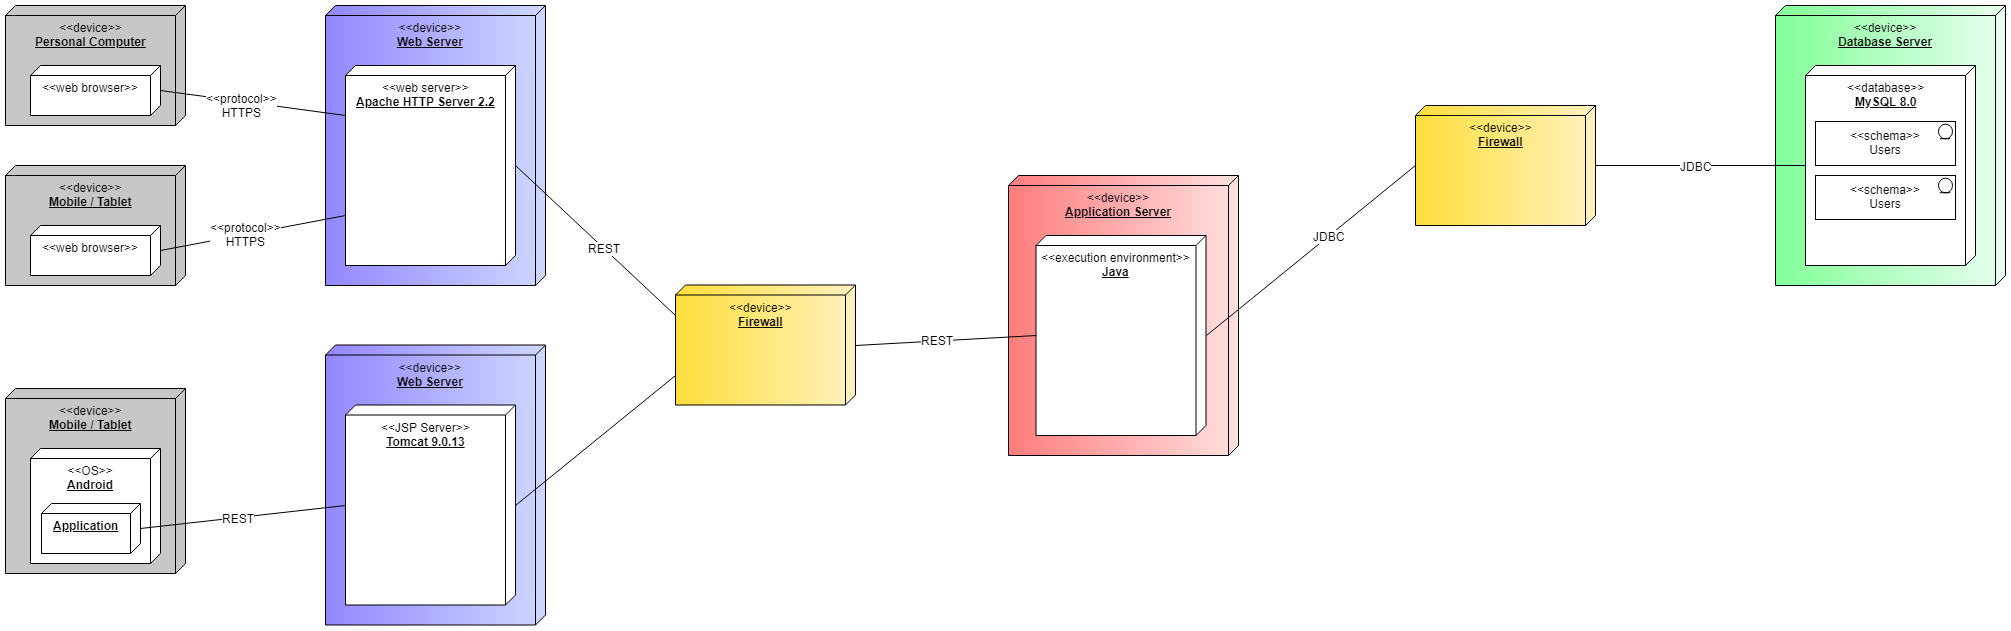
\includegraphics[angle=90, height=0.9\textheight]{deploymentDiagram.png}
	\caption{Track4Run Components}
\end{figure}
\FloatBarrier

\subsection{Runtime View}
- Auth
- One-shot req
- Subscription req
- New data arrives

\subsection{Component Interfaces}
\subsection{Selected Architectural Styles and Patterns}
- stateless
- microservice
- monolithic
- token auth
- loose coupling
- event driven and message queues
- server side service discovery
\subsection{Other Design Decisions}
- NOSQL DB
- JWT
- REST
- RabbitMQ

\newpage

\section{User Interface Design}
// TODO

\newpage

\section{Requirements Traceability}
\begin{table}
\begin{adjustwidth}{-4cm}{}
\captionsetup{justification=centering}
\caption{Data4Help requirements traceability matrix}
  \label{tab:table1}
\begin{tabular}{|l||l|l|l|l|l|l|l|l|l|l|l|l|l|l|l|}
\hline
\cellcolor[HTML]{EFEFEF}                      & \cellcolor[HTML]{EFEFEF} R1 & \cellcolor[HTML]{EFEFEF} R2 & \cellcolor[HTML]{EFEFEF} R3 & \cellcolor[HTML]{EFEFEF} R4 & \cellcolor[HTML]{EFEFEF} R5 & \cellcolor[HTML]{EFEFEF} R6 & \cellcolor[HTML]{EFEFEF} R7 & \cellcolor[HTML]{EFEFEF} R8 & \cellcolor[HTML]{EFEFEF} R9 &\cellcolor[HTML]{EFEFEF}  R10 & \cellcolor[HTML]{EFEFEF} R11 & \cellcolor[HTML]{EFEFEF} R12 & \cellcolor[HTML]{EFEFEF} R13 & \cellcolor[HTML]{EFEFEF} R14 & \cellcolor[HTML]{EFEFEF} R15\\ \hline \hline
\cellcolor[HTML]{EFEFEF}AuthenticationService & $\checkmark$  & $\checkmark$  & $\checkmark$  &    & $\checkmark$  & $\checkmark$  & $\checkmark$  &    &    &     &     &     &     &     & \\ \hline
\cellcolor[HTML]{EFEFEF}DataSourceManager     &    &    &    & $\checkmark$  &    &    &    &    &    &     &     &     &     &     & \\ \hline
\cellcolor[HTML]{EFEFEF}Data Receiver         &    &    &    &    & $\checkmark$  &    &    &    &    &     &     &     & $\checkmark$   &     & \\ \hline
\cellcolor[HTML]{EFEFEF} SingleDataManager    &    &    &    &    &    &    &    & $\checkmark$  &    &     &     &     &     &     & \\ \hline
\cellcolor[HTML]{EFEFEF} GroupDataManagement  &    &    &    &    &    &    &    &    & $\checkmark$  & $\checkmark$   &     &     &     &     & $\checkmark$ \\ \hline
\cellcolor[HTML]{EFEFEF} SubscriptionService  &    &    &    &    &    &    &    &    &    &     & $\checkmark$   &     & $\checkmark$   &     & \\ \hline
\cellcolor[HTML]{EFEFEF} RequestManager       &    &    &    &    &    &    &    &    &    &     &     & $\checkmark$   &     & $\checkmark$   & $\checkmark$ \\ \hline
\cellcolor[HTML]{EFEFEF} DataSender           &    &    &    &    &    &    &    &    &    &     &     &     & $\checkmark$   &     & \\ \hline
\end{tabular}
\end{adjustwidth}
\end{table}


\begin{table}
\begin{adjustwidth}{-4cm}{}
\captionsetup{justification=centering}
\caption{AutomatedSOS requirements traceability matrix}
  \label{tab:table2}
\begin{tabular}{|l||l|l|l|l|l|l|l|l|}
\hline
\cellcolor[HTML]{EFEFEF}                      & \cellcolor[HTML]{EFEFEF} R16 & \cellcolor[HTML]{EFEFEF} R17 & \cellcolor[HTML]{EFEFEF} R18 & \cellcolor[HTML]{EFEFEF} R19 & \cellcolor[HTML]{EFEFEF} R20 & \cellcolor[HTML]{EFEFEF} R21 & \cellcolor[HTML]{EFEFEF} R22 & \cellcolor[HTML]{EFEFEF} R23 \\ \hline \hline
\cellcolor[HTML]{EFEFEF}AuthenticationService & $\checkmark$  &    &    &   &   &   &    &    \\ \hline
\cellcolor[HTML]{EFEFEF}LoginService     &  $\checkmark$  &       &   &    & $\checkmark$   &    &    &    \\ \hline
\cellcolor[HTML]{EFEFEF}DataRetrievalService         &    & $\checkmark$     &    &   &  $\checkmark$  &    &    &   \\ \hline
\cellcolor[HTML]{EFEFEF} Monitoring Service    &    &   $\checkmark$ &      &    &    &  $\checkmark$  & $\checkmark$  &  $\checkmark$  \\ \hline
\cellcolor[HTML]{EFEFEF} ThresholdSettingService  &    &       &  $\checkmark$  &  $\checkmark$  &    &    &    &    \\ \hline
\cellcolor[HTML]{EFEFEF} ClientApplication  &    &    &       &    &    &  $\checkmark$  &  $\checkmark$  &     \\ \hline
\end{tabular}
\end{adjustwidth}
\end{table}

\begin{table}
\begin{adjustwidth}{-4cm}{}
\captionsetup{justification=centering}
\caption{Track4Run requirements traceability matrix}
  \label{tab:table3}
\begin{tabular}{|l||l|l|l|l|l|l|l|l|l|l|l|}
\hline
\cellcolor[HTML]{EFEFEF}                      & \cellcolor[HTML]{EFEFEF} R24 & \cellcolor[HTML]{EFEFEF} R25 & \cellcolor[HTML]{EFEFEF} R26 & \cellcolor[HTML]{EFEFEF} R27 & \cellcolor[HTML]{EFEFEF} R28 & \cellcolor[HTML]{EFEFEF} R29 & \cellcolor[HTML]{EFEFEF} R30 & \cellcolor[HTML]{EFEFEF} R31 & \cellcolor[HTML]{EFEFEF} R32 & \cellcolor[HTML]{EFEFEF} R33 & \cellcolor[HTML]{EFEFEF} R34\\ \hline \hline
\cellcolor[HTML]{EFEFEF} AuthenticationService & $\checkmark$  &   &  &    &   &   &   &    &   &   &   \\ \hline
\cellcolor[HTML]{EFEFEF}LoginService     &  $\checkmark$  &    &    &   &    &    &    &    &   &   &  \\ \hline
\cellcolor[HTML]{EFEFEF}RunCreationManagement         &    & $\checkmark$   &  $\checkmark$  &  $\checkmark$  & $\checkmark$  &  $\checkmark$  &    &    &   &   & \\ \hline
\cellcolor[HTML]{EFEFEF} RunSearchService    &    &    &    &    &    &    &  $\checkmark$ &   &  & $\checkmark$ & \\ \hline
\cellcolor[HTML]{EFEFEF} EnrollmentManager  &    &    &    &    &    &    & $\checkmark$   &  $\checkmark$  &   &   & \\ \hline
\cellcolor[HTML]{EFEFEF} SpectatorService  &    &    &    &    &   &    &    &    &   &  $\checkmark$ & \\ \hline
\cellcolor[HTML]{EFEFEF} DataRetrievalService  &    &    &    &    &    &    &    &    &  $\checkmark$   &   &  \\ \hline
\cellcolor[HTML]{EFEFEF} ClientApplication  &    &    &    &    &    &    &    &    &     &   & $\checkmark$ \\ \hline
\end{tabular}
\end{adjustwidth}
\end{table}

\newpage

\section{Implementation, Integration and Test Plan}
\subsection{Implementation Plan}
In the implementation phase of our project we decided to follow a bottom-up strategy. In particular, starting from the Data4Help subsystem, we will implement each component separately and then perform unit tests on it. By adopting this strategy we incrementally develop working components.
As it concerns the implementation order, we decided to start from the Data4Help back-end module, since we think is the most critical one because the other two subsystems work on top of it.
In a second time, developer SDKs should be completed before the other two subsystem's back-end development can be carried out.
Finally, we can integrate front-ends in all our systems.
The order could be the following:

\begin{enumerate}
    \item Data4Help back-end
    \item Third Party SDK
    \item Data Source SDK
    \item Automated SOS and Track4Run back-end
    \item Data4Help front-end
    \item AutomatedSOS and Track4Run front-end
\end{enumerate}


The following diagrams are meant to provide a more precise overview of our implementation plan.

\subsubsection{Data4Help Basic Back-End}

The first components to be developed should be the ones that guarantee the basic back-end functions of the Data4Help, which means all the services that are related to data acquisition and data requests. 

Here is a digram representing a possible order in which these components should be developed. As already stated, after each development phase a \textit{Unit Test} phase and an \textit{Integration Test} phase should follow, in order to validate the new component and verify its integration with the previously developed system.

\FloatBarrier
\begin{figure}[!h]
	\centering
	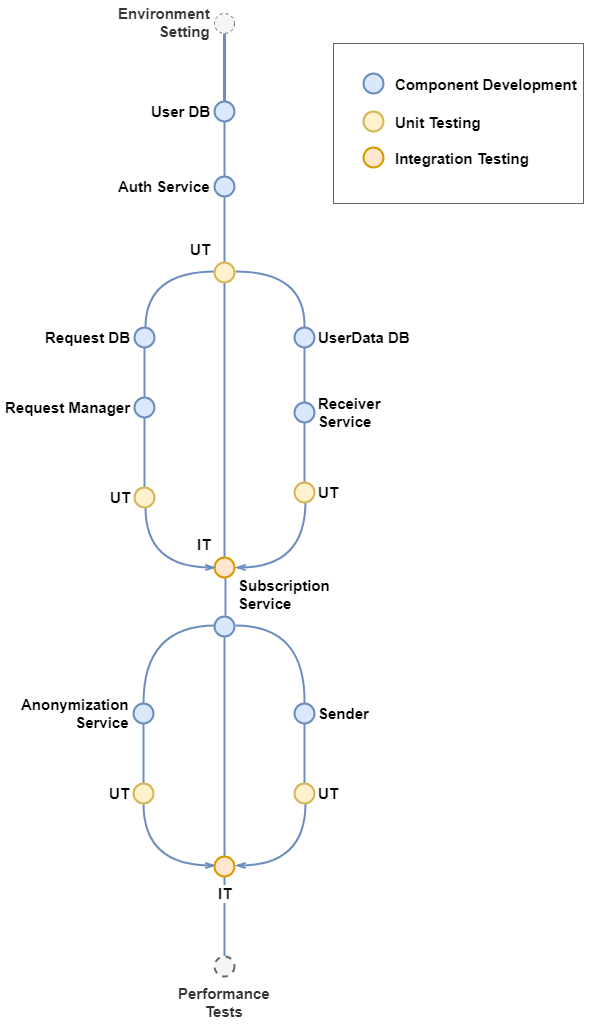
\includegraphics[width=0.7\columnwidth]{d4h_dev.png}
	\caption{Data4Help Development Plan}
\end{figure}
\FloatBarrier

\subsubsection{Developer's SDKs}
The Third Party SDK and Data Sources SDK must be carried out after Data4Help basic back-end is completed and before developing other back-ends. This will guarantee the AutomatedSOS and Track4Run subsystems to be able to properly interact with the Data4Help APIs.

In particular, there is no dependency between the two SDKs, but certainly the Third-Party SDK is the most important one in this phase, since AutomatedSOS and Data4Help development depend on it. In case this SDK's development is found to take a long time, the two subsystem's development can start independently, and integrate the SDKs in a second moment.

\subsubsection{AutomatedSOS and Track4Run Back-Ends}
After the SDKs are developed, the remaining two subsystems' back-ends can be developed in a fully parallel line. Like in the case of Data4Help, an incremental approach is recommended in these development phases, and Unit and Integration test should be performed at every step.

\FloatBarrier
\begin{figure}[!h]
	\centering
	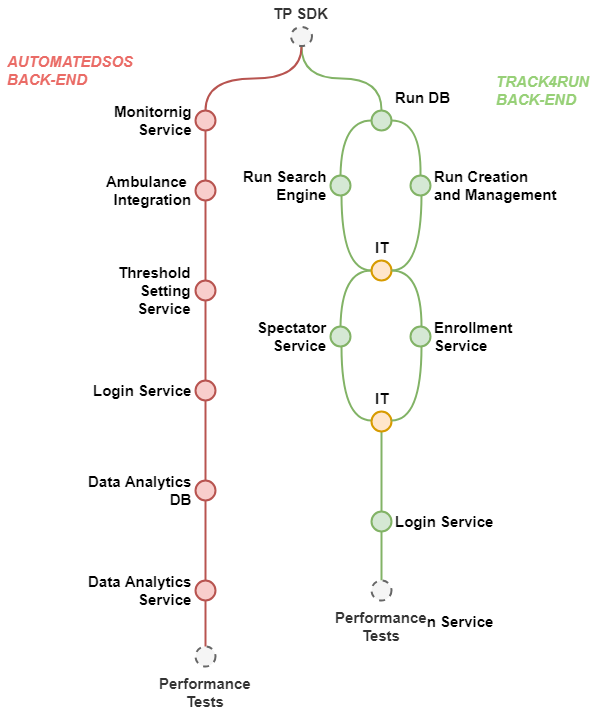
\includegraphics[width=0.9\columnwidth]{other_be_dev.png}
	\caption{Data4Help Development Plan}
\end{figure}
\FloatBarrier

\subsubsection{Front-Ends and External Services Integration}
Finally, the front-ends can be developed and the subsystems can be integrated with the external services. Each front-end is obviously independent from the others, and the external service integration can as well be performed separately for each subsystem.

\begin{itemize}
	\item \textbf{Data4Help}
\end{itemize}

\FloatBarrier	
\begin{figure*}[ht!]	
	\centering	
	\begin{subfigure}[t]{0.5\textwidth}	
		\centering	
		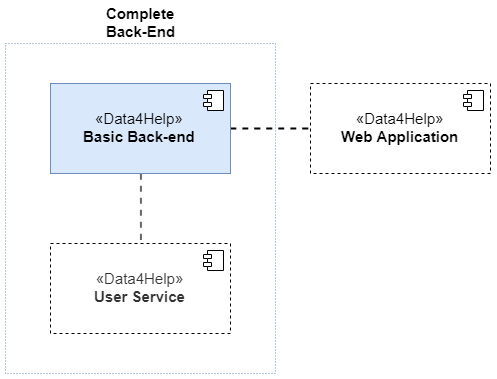
\includegraphics[width=\columnwidth]{d4h_int1.png}	
		\caption{Stage I}	
	\end{subfigure}%	
	~ \vspace{20px}	
	\begin{subfigure}[t]{0.5\textwidth}	
		\centering	
		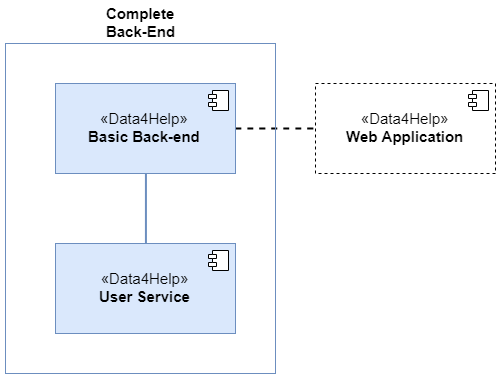
\includegraphics[width=\columnwidth]{d4h_int2.png}	
		\caption{Stage II}	
	\end{subfigure}	
	\begin{subfigure}[t]{0.5\textwidth}	
		\centering	
		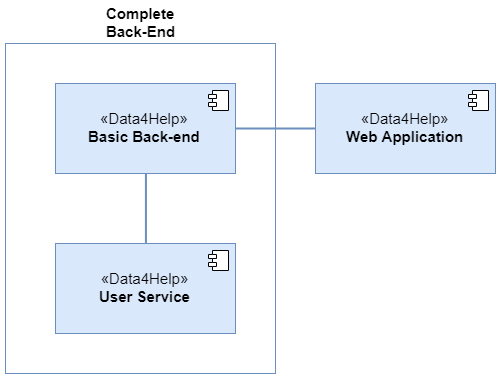
\includegraphics[width=\columnwidth]{d4h_int3.png}	
		\caption{Stage III}	
	\end{subfigure}	
	
	\caption{Data4Help Front-End Integration Steps}	
\end{figure*}	

\FloatBarrier
	
\begin{itemize}
	\item \textbf{AutomatedSOS}
\end{itemize}


\FloatBarrier
\begin{figure*}[ht!]	
	\centering	
	\begin{subfigure}[t]{0.5\textwidth}	
		\centering	
		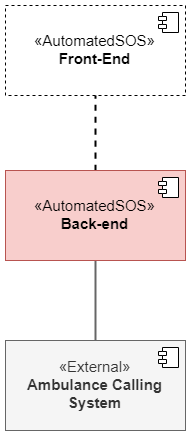
\includegraphics[width=0.5\columnwidth]{autosos_int1.png}	
		\caption{Stage I}	
	\end{subfigure}%	
	~ \vspace{20px}	
	\begin{subfigure}[t]{0.5\textwidth}	
		\centering	
		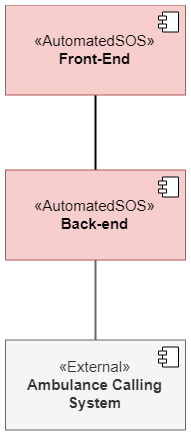
\includegraphics[width=0.5\columnwidth]{autosos_int2.png}	
		\caption{Stage II}	
	\end{subfigure}	
	\caption{AutomatedSOS Final Integration Steps}	
\end{figure*}	

\FloatBarrier

\begin{itemize}
	\item \textbf{Track4Run}
\end{itemize}


\FloatBarrier
\begin{figure*}[ht!]	
	\centering	
	\begin{subfigure}[t]{0.3\textwidth}	
		\centering	
		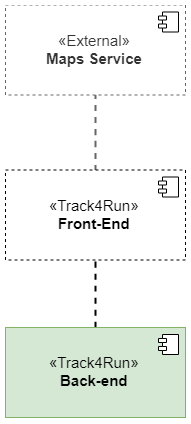
\includegraphics[width=0.8\columnwidth]{t4r_int1.png}	
		\caption{Stage I}	
	\end{subfigure}%		
	~ \vspace{20px}	
	\begin{subfigure}[t]{0.3\textwidth}	
		\centering	
		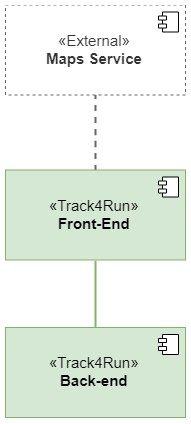
\includegraphics[width=0.8\columnwidth]{t4r_int2.png}	
		\caption{Stage II}	
	\end{subfigure}
	~ \vspace{20px}
	\begin{subfigure}[t]{0.3\textwidth}	
		\centering	
		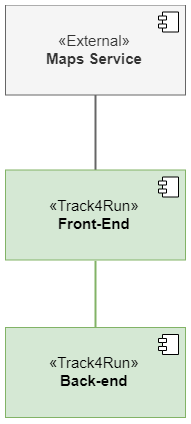
\includegraphics[width=0.8\columnwidth]{t4r_int3.png}	
		\caption{Stage III}	
	\end{subfigure}	
	
	\caption{Track4Run Final Integration Steps}	
\end{figure*}	
\FloatBarrier

\subsection{Integration and Testing}
\subsubsection{Integration Testing Strategy}
With respect to the integration between developed components, we decided to follow a \textit{continuous integration} strategy: as soon as a first version of a component is released, we need to test it and then integrate it with the already existing components of the system. This strategy has been chosen because it enables the developers to have many checkpoints where they can test their product and makes it easy to found bugs early in the development of the system, so that if things break, they break small.

 
Once each back-end have been completely developed and integrated, it's also highly recommended to carry out a system testing process. In particular:

\begin{itemize}
    \item \textbf{Performance Testing:} in each system, we need to monitor the responsiveness of the services with respect to incoming requests. In particular, Data4Help should be very fast in managing new data samples to guarantee a fluid service to the third-parties. In addition, AutomatedSOS needs to be extremely fast in detecting and responding to an emergency. Lastly, Track4Run user experience is heavily influenced by the back-end performances, which should be for this reason flawless.
    \item \textbf{Load Testing:} 
    \item \textbf{Stress Testing:}
\end{itemize}

\subsubsection{Entry Criteria}
As stated above, continuous integration forces the testing phase to start as soon as a component is merged with the main product. However, it is necessary to be sure that a correct environment is setup before integration can be effectively carried out. In particular, in case of Data4Help we need the following components:

\begin{itemize}
    \item \textit{Microservices Containers:} needed to deploy a distributed microservice cluster
    \item \textit{API Gateway:} provides a unified interface for redirecting service requests
    \item \textit{Message Queue Server:} used for inter-service asynchronous communication
    \item \textit{Service Registry:} holds the reference to all the microservices of the cluster
    \item \textit{DataBase Managment System:} provides entrypoints to the DataBases
\end{itemize}

For AutomatedSOS and Track4Run instead we need the web server and firewalls to be correctly set-up and the \textit{Third-Party SDK} to be available and already tested against the Data4Help request APIs.

\subsubsection{Elements to be Integrated}
As seen in the development plan, we can divide our components in groups considering the existing dependencies between them.

// TODO

\subsubsection{Sequence of Component/Function Integration}
Since we adopted a continuous integration strategy, the integration phase runs in parallel  with the implementation phase, which is carefully described in the previous diagrams.


\newpage

\section{Effort Spent}
\vspace{0.5cm}

\begin{center}
    \begin{tabu} to 0.8\textwidth { | X[c] X[c] | }
         \hline
         \multicolumn{2}{|c|}{Marco Gelli}\\
         \tabuphantomline
         \hline
         Component Brainstorming & 4 Hours \\
         Requirements Traceability & 4 Hours \\
         Subject 3 & Hours \\
         Subject 4 & Hours \\
         Subject 5 & Hours \\
         Subject 6 & Hours \\
        \hline
    \end{tabu}
\end{center}

\vspace{0.5cm}

\begin{center}
    \begin{tabu} to 0.8\textwidth { | X[c] X[c] | }
         \hline
         \multicolumn{2}{|c|}{Alvise de'Faveri Tron} \\
         \hline
         Component Brainstorming & 4 Hours \\
         Requirements Traceability & 5 Hours \\
         Subject 3 & Hours \\
         Subject 4 & Hours \\
         Subject 5 & Hours \\
         Subject 6 & Hours \\
        \hline
    \end{tabu}
\end{center}

\vspace{0.5cm}

\begin{center}
    \begin{tabu} to 0.8\textwidth { | X[c] X[c] | }
         \hline
         \multicolumn{2}{|c|}{Andrea Biscontini} \\
         \hline
        Requirements Traceability & 5 Hours \\
         Subject 2 & Hours \\
         Subject 3 & Hours \\
         Subject 4 & Hours \\
         Subject 5 & Hours \\
         Subject 6 & Hours \\
        \hline
    \end{tabu}
\end{center}


\newpage

\section{References}
// TODO

\end{document}